\documentclass[12pt,a4paper]{article}

% ── Packages ─────────────────────────────────────────────────────────────────
\usepackage[utf8]{inputenc}
\usepackage[T1]{fontenc}
\usepackage[margin=2.5cm]{geometry}
\usepackage{amsmath, amssymb}
\usepackage{graphicx}
\usepackage{booktabs}
\usepackage{enumitem}
\usepackage{titlesec}
\usepackage{titletoc}
\usepackage{parskip}
\usepackage{soul, xcolor}
\usepackage{fancyhdr}
\usepackage{mdframed}
\usepackage{listings}
\usepackage{tikz}
\usetikzlibrary{shapes.geometric, arrows.meta, positioning}
\usepackage[colorlinks=true, linkcolor=indigo, urlcolor=indigo, citecolor=indigo]{hyperref}
\usepackage{multicol}
\usepackage{array}
\usepackage{longtable}

% ── Colours ──────────────────────────────────────────────────────────────────
\definecolor{indigo}{RGB}{79,70,229}
\definecolor{emerald}{RGB}{16,185,129}
\definecolor{amber}{RGB}{245,158,11}
\definecolor{rose}{RGB}{225,29,72}
\definecolor{slate}{RGB}{71,85,105}
\definecolor{codebg}{RGB}{15,23,42}
\definecolor{codetext}{RGB}{148,163,184}

% ── Section formatting ────────────────────────────────────────────────────────
\titleformat{\section}{\large\bfseries\color{indigo}}{}{0em}{}[\titlerule]
\titleformat{\subsection}{\normalsize\bfseries\color{slate}}{}{0em}{}
\titleformat{\subsubsection}{\normalsize\itshape\color{slate}}{}{0em}{}

% ── Header / footer ───────────────────────────────────────────────────────────
\pagestyle{fancy}
\fancyhf{}
\fancyhead[L]{\small\color{slate} Layout OCR — Phase 2 Report}
\fancyhead[R]{\small\color{slate} Professional Practices in IT}
\fancyfoot[C]{\small\color{slate}\thepage}
\renewcommand{\headrulewidth}{0.4pt}

% ── Code listing style ────────────────────────────────────────────────────────
\lstset{
  basicstyle=\ttfamily\footnotesize\color{codetext},
  backgroundcolor=\color{codebg},
  frame=single, rulecolor=\color{slate},
  breaklines=true, keepspaces=true,
  keywordstyle=\color{indigo}\bfseries,
  commentstyle=\color{emerald},
  stringstyle=\color{amber},
}

% ── Info box environment ──────────────────────────────────────────────────────
\newmdenv[linecolor=indigo, linewidth=1.2pt, backgroundcolor=indigo!5,
  innerleftmargin=10pt, innerrightmargin=10pt,
  innertopmargin=8pt, innerbottommargin=8pt]{infobox}

\newmdenv[linecolor=emerald, linewidth=1.2pt, backgroundcolor=emerald!5,
  innerleftmargin=10pt, innerrightmargin=10pt,
  innertopmargin=8pt, innerbottommargin=8pt]{successbox}

\newmdenv[linecolor=amber, linewidth=1.2pt, backgroundcolor=amber!5,
  innerleftmargin=10pt, innerrightmargin=10pt,
  innertopmargin=8pt, innerbottommargin=8pt]{warningbox}


% ─────────────────────────────────────────────────────────────────────────────
\begin{document}

% ── Title Page ────────────────────────────────────────────────────────────────
\begin{titlepage}
  \centering
  \vspace*{2cm}
  {\Huge\bfseries\color{indigo} Layout OCR}\\[0.4cm]
  {\Large\color{slate} Agentic Document Transcription System}\\[0.2cm]
  {\large\color{slate} Phase 2 Technical \& Professional Practices Report}\\[3cm]

  \begin{tabular}{rl}
    \textbf{Course:}    & Professional Practices in IT \\[0.4em]
    \textbf{Phase:}     & 2 — Transformation into a Purely Agentic System \\[0.4em]
    \textbf{Alignment:} & CLO 4, CLO 5, CLO 6, CLO 8 (NCEAC) \\[0.4em]
    \textbf{Date:}      & May 2026 \\
  \end{tabular}

  \vfill
  {\small\color{slate} Confidential Academic Document — Professional Practices in IT}
\end{titlepage}

\newpage
\tableofcontents
\newpage


% =============================================================================
\section{Phase 1 Recap}
% =============================================================================

\subsection{Problem Statement}
Students, researchers, and professionals regularly produce handwritten notes, lecture slides, and
annotated documents that are difficult to digitise accurately. Existing OCR tools either produce
plain text (losing all structure) or require expensive proprietary software. The goal of
\textbf{Layout OCR} was to bridge this gap by producing a structured, editable
\LaTeX{} document from a single photograph.

\subsection{Target Users}
\begin{itemize}[noitemsep]
  \item University students converting handwritten notes into shareable \LaTeX{} documents
  \item Academics archiving annotated lecture material
  \item Professionals digitising whiteboard sketches with embedded diagrams
\end{itemize}

\subsection{Phase 1 Technology Stack}
\begin{center}
\begin{tabular}{ll}
  \toprule
  \textbf{Layer} & \textbf{Technology} \\
  \midrule
  Frontend        & React 18 + TypeScript + Tailwind CSS + Vite \\
  Backend API     & Python 3.12 + FastAPI + Uvicorn \\
  AI Model        & Anthropic Claude Sonnet 4.6 (via REST API) \\
  Output          & \LaTeX{} (.tex) + cropped images (ZIP) \\
  PDF Compilation & Tectonic (\LaTeX{} engine) \\
  \bottomrule
\end{tabular}
\end{center}

\subsection{Phase 1 Features}
\begin{itemize}[noitemsep]
  \item Upload image (drag-and-drop or file picker)
  \item Single-pass AI extraction of headings, paragraphs, lists, tables, formulas, and images
  \item Download ZIP containing \texttt{.tex} source and cropped image assets
  \item Open directly in Overleaf via HTTP POST form
  \item Server-side PDF compilation and download
  \item Session history with star-rating feedback
\end{itemize}


% =============================================================================
\section{Computing as a Formal Profession}
% =============================================================================

Software development is not merely a technical trade — it is a \textbf{formal profession} governed
by codes of conduct, ethical obligations, and legal frameworks comparable to medicine or law.

\subsection{Professional Responsibilities in Layout OCR}

\begin{itemize}[noitemsep]
  \item \textbf{Responsibility toward users:} The system processes potentially sensitive academic
    documents. Users must be able to trust that their content is not retained beyond the session,
    misused, or exposed to third parties.

  \item \textbf{Responsibility toward society:} Automating document transcription must not
    facilitate plagiarism or misrepresentation of authorship. The tool produces \LaTeX{} — it is
    the user's professional responsibility to correctly attribute source material.

  \item \textbf{Responsibility toward data:} Images uploaded may contain personal information
    (exam answers, private notes). The system uses in-memory session storage with no persistent
    disk logging of content beyond the active session.
\end{itemize}

\subsection{Why This Matters}
The transition from Phase 1 (a static tool) to Phase 2 (an autonomous agentic system) amplifies
professional responsibility significantly. When a system makes decisions autonomously — choosing
what to extract, what quality threshold is acceptable, and when to iterate — the developer becomes
accountable for those decisions in a way that a simple file-format converter does not require.


% =============================================================================
\section{Ethics vs.\ Morals in System Design}
% =============================================================================

\begin{center}
\begin{tabular}{p{5cm}p{8cm}}
  \toprule
  \textbf{Concept} & \textbf{Application to Layout OCR} \\
  \midrule
  \textbf{Morals} (personal beliefs) &
    A developer might personally believe that any AI that alters user-submitted text is
    acceptable. However, this personal view is irrelevant when professional standards and user
    trust are at stake. \\[0.6em]
  \textbf{Ethics} (professional standards) &
    Professionally, the system must be transparent about what it has changed (spell-correction,
    layout inference) and provide the user full override capability before any output is
    finalised. \\
  \bottomrule
\end{tabular}
\end{center}

\subsection{Design Decisions Reflecting Professional Ethics}

The \textbf{Human-in-the-Loop preview step} (Section~\ref{sec:hitl}) is the primary ethical
safeguard. Before any \LaTeX{} is generated, the user sees every extracted element and can edit,
delete, or retype content. This was a deliberate \emph{professional} decision, not a personal
preference — it prevents the AI from silently corrupting academic content.


% =============================================================================
\section{Professional Ethics: Responsibility in Code Quality, Security, and User Safety}
% =============================================================================

\subsection{Code Quality}
\begin{itemize}[noitemsep]
  \item Structured JSON output enforced via Claude \texttt{tool\_use} with forced tool choice —
    prevents the model from returning free-form text that could break downstream parsing.
  \item All blocking I/O (AI calls, image processing) runs in \texttt{asyncio.to\_thread()} to
    keep the FastAPI event loop responsive and prevent server hangs.
  \item Image crops use the \emph{original} high-resolution image, not the resized API copy,
    ensuring output quality is not degraded.
\end{itemize}

\subsection{Security Considerations}
\begin{itemize}[noitemsep]
  \item The API key (\texttt{ANTHROPIC\_API\_KEY}) is loaded from a \texttt{.env} file via
    \texttt{python-dotenv} and never exposed to the frontend or logged.
  \item File uploads are validated for MIME type (\texttt{image/*}) before processing.
  \item Temporary files are deleted immediately after extraction; \texttt{tempfile.NamedTemporaryFile}
    with \texttt{delete=False} is used with explicit cleanup in a \texttt{finally} block.
  \item Sessions are stored in-memory (not on disk) and keyed by UUID4, making brute-force
    enumeration infeasible.
\end{itemize}

\subsection{User Safety}
\begin{itemize}[noitemsep]
  \item The preview step ensures the user approves all AI decisions before output is generated.
  \item The Verification Agent (Agent 3) provides an independent post-generation quality score,
    allowing the user to make an informed decision before using the output.
  \item LaTeX compilation errors are surfaced with the full tectonic log, not silently swallowed.
\end{itemize}


% =============================================================================
\section{Ethical Decision Making}
% =============================================================================

\subsection{Identified Ethical Decision: Speed vs.\ Quality}

During Phase 2 development, a key trade-off arose: should the system perform a single fast
extraction or run multiple agent passes (slower but more accurate)?

\begin{center}
\begin{tabular}{lp{5cm}p{5cm}}
  \toprule
  & \textbf{Speed (1 pass)} & \textbf{Quality (multi-pass)} \\
  \midrule
  User impact   & Faster feedback & More accurate output \\
  Trust impact  & Risk of silent errors in academic work & Higher confidence in results \\
  Resource cost & Lower API cost & Higher API cost \\
  Decision      & & \textbf{Chosen: multi-pass with convergence} \\
  \bottomrule
\end{tabular}
\end{center}

\textbf{Justification:} For academic document transcription, an error in a formula, table, or
diagram is worse than a slower response. The 4-step model guided this decision:

\begin{enumerate}[noitemsep]
  \item \textbf{Identify the issue:} Single-pass OCR can miss content or misread handwriting.
  \item \textbf{Analyse stakeholders:} Students submitting AI-transcribed notes are responsible
    for accuracy; errors could constitute unintentional academic misconduct.
  \item \textbf{Evaluate alternatives:} Single pass (fast, risky) vs.\ multi-pass with critic
    (slower, reliable). A user override is provided in both cases.
  \item \textbf{Make justified decision:} Multi-pass was selected with a maximum of 4 passes and
    real-time progress streaming so the user is never left uncertain.
\end{enumerate}

\subsection{Cybersecurity Consideration: Vulnerability Disclosure}
The Anthropic API key is the most sensitive credential in this system. A disclosure policy was
implemented: the key is never serialised into logs, never transmitted to the frontend, and the
\texttt{.env} file is listed in \texttt{.gitignore} to prevent accidental public disclosure.


% =============================================================================
\section{Ethical Theories \& Human-Centred Design}
% =============================================================================

\subsection{Utilitarianism}
The multi-agent refinement loop produces the \emph{greatest good for the greatest number} of
users: a higher-quality transcription benefits every user, even though it costs more API calls.
The convergence condition (score $\geq 85$, no critical issues) was chosen to balance quality
against unnecessary computation.

\subsection{Deontology}
Regardless of outcome, the system has a \emph{duty} to be transparent. Every AI decision — each
extraction pass, each critique score, each acceptance decision — is streamed to the user in
real-time via Server-Sent Events. The user always knows what the agents are doing.

\subsection{Human-Centred Design}
\begin{itemize}[noitemsep]
  \item \textbf{Risks of addictive automation:} A system that silently produces ``good enough''
    output discourages critical review. The explicit preview step and verification score
    encourage active user engagement rather than passive acceptance.
  \item \textbf{Override at every stage:} The user can edit any extracted element, delete any
    element, change element types, and adjust formatting before committing to LaTeX generation.
  \item \textbf{Explainability:} Agent 2's critique issues (severity, description, suggested fix)
    and Agent 3's verification report are shown in the UI so users understand \emph{why} the AI
    made its decisions.
\end{itemize}


% =============================================================================
\section{ACM / IEEE Code of Ethics}
% =============================================================================

\subsection{Principles Followed}

\begin{enumerate}[noitemsep]
  \item \textbf{ACM 1.1 — Contribute to society and human well-being:}
    Layout OCR makes academic document digitisation accessible without requiring expensive
    proprietary tools or specialised LaTeX knowledge.

  \item \textbf{ACM 2.1 — Strive to achieve high quality:}
    The multi-agent critique loop directly instantiates this principle — Agent 2 exists
    specifically to enforce quality standards that Agent 1 might not achieve in isolation.

  \item \textbf{IEEE 1.03 — Approve software only if safe:}
    The Human-in-the-Loop preview step ensures no LaTeX is generated without explicit user
    approval. The system never automatically delivers output.
\end{enumerate}

\subsection{Principle Potentially Violated}

\textbf{ACM 1.6 — Respect privacy:} The system sends user-uploaded images to a third-party API
(Anthropic). Users are not explicitly informed of this within the UI. Mitigation: images are
sent only for processing, are not retained by the API beyond the request lifetime (per
Anthropic's data policy), and no personal data is persisted server-side beyond the active
session.


% =============================================================================
\section{Software Development \& Industry Practices}
% =============================================================================

\subsection{Project vs.\ Industry Workflow Comparison}

\begin{center}
\begin{tabular}{lp{5cm}p{5cm}}
  \toprule
  \textbf{Practice} & \textbf{This Project} & \textbf{Industry Standard} \\
  \midrule
  Version control   & Git (single branch, commit history) & Git Flow / trunk-based \\
  Communication     & Developer + end user (student context) & Scrum, sprint reviews \\
  Testing           & Manual end-to-end; TypeScript type-check & CI/CD + automated unit/integration tests \\
  AI ethics         & Prompt design, human override, explainability & Responsible AI frameworks, red-teaming \\
  AI bias           & Multi-pass critique reduces single-model bias & Adversarial testing, diverse training data \\
  \bottomrule
\end{tabular}
\end{center}

\subsection{AI Ethics \& Bias in Prompt Engineering}

A single AI model can exhibit systematic biases: consistently misreading certain handwriting
styles, preferring certain element types, or dropping content that is less common in its
training data (e.g.\ diagrams). The two-agent design partially mitigates this:
Agent 1 (Extractor) and Agent 2 (Critic) are the \emph{same model} but given different
\emph{roles and incentives} — the critic is explicitly instructed to be ``strict'' and treat
missing images as critical failures, counteracting the extractor's tendency to omit them.


% =============================================================================
\section{Trends in IT \& Agentic Systems}
% =============================================================================

The industry is undergoing a shift from \textbf{static software tools} to
\textbf{autonomous agent systems}. Key trends that motivated Phase 2:

\begin{itemize}[noitemsep]
  \item \textbf{Rise of LLM-based agents:} Systems like AutoGPT, Claude's tool-use API, and
    OpenAI Assistants demonstrate that LLMs can self-direct multi-step tasks with structured
    tool outputs — the foundation of this project's agentic loop.

  \item \textbf{Critique-and-refine patterns:} Constitutional AI, RLHF, and agent frameworks
    such as LangGraph use the same principle: a second model (or the same model in a critic role)
    reviews and improves the output of a generator. This project independently implements this
    pattern.

  \item \textbf{Human-in-the-loop as a safety standard:} Industry consensus (e.g.\ EU AI Act,
    IEEE Ethically Aligned Design) is converging on mandatory human oversight for high-stakes
    AI outputs. Academic document transcription qualifies as high-stakes.

  \item \textbf{Streaming UX:} Server-Sent Events and real-time progress interfaces are
    increasingly expected for any AI workflow that takes more than a second. OpenAI, Anthropic,
    and Gemini all provide streaming APIs for this reason.
\end{itemize}


% =============================================================================
\section{Agentic Transformation}
% =============================================================================

\subsection{Technical Limitations of Phase 1}

\begin{center}
\begin{tabular}{lp{10cm}}
  \toprule
  \textbf{Limitation} & \textbf{Description} \\
  \midrule
  Static logic      & A single API call with no feedback loop; if the first extraction was poor,
                      there was no mechanism to improve it. \\
  No autonomy       & The system could not decide whether its output was adequate or request a
                      second opinion. \\
  No intelligence   & No reasoning about quality, completeness, or correctness of the
                      extraction. \\
  Image fragility   & Images were sometimes dropped silently; no validation that all visual
                      content was captured. \\
  \bottomrule
\end{tabular}
\end{center}

\subsection{Gap Analysis: Why Phase 1 Was Not Agentic}

An agentic system must exhibit \textbf{Perception, Decision-making, Action, and Learning}.
Phase 1 had only rudimentary Perception (sending the image to an API) and Action (returning a
response). It had \emph{no} decision-making (was the output good enough?) and \emph{no} learning
(could it improve given feedback?). It was a pipeline, not an agent.

\subsection{Agentic Vision: Tool $\rightarrow$ Agent, Reactive $\rightarrow$ Proactive}

\begin{center}
\begin{tabular}{lll}
  \toprule
  \textbf{Dimension} & \textbf{Phase 1 (Tool)} & \textbf{Phase 2 (Agent)} \\
  \midrule
  Control      & User-driven (request/response) & System-driven (autonomous loop) \\
  Intelligence & Static (single prompt)         & Adaptive (critique $\rightarrow$ refine) \\
  Behaviour    & Reactive (responds to input)   & Proactive (iterates until quality gate) \\
  Memory       & None                           & Short-term (iteration log) \\
  \bottomrule
\end{tabular}
\end{center}


% =============================================================================
\section{Agent Architecture}
\label{sec:architecture}
% =============================================================================

\subsection{System Overview}

The Phase 2 system implements a \textbf{goal-based, learning agent architecture} with three
specialised sub-agents operating in a directed loop.

\begin{center}
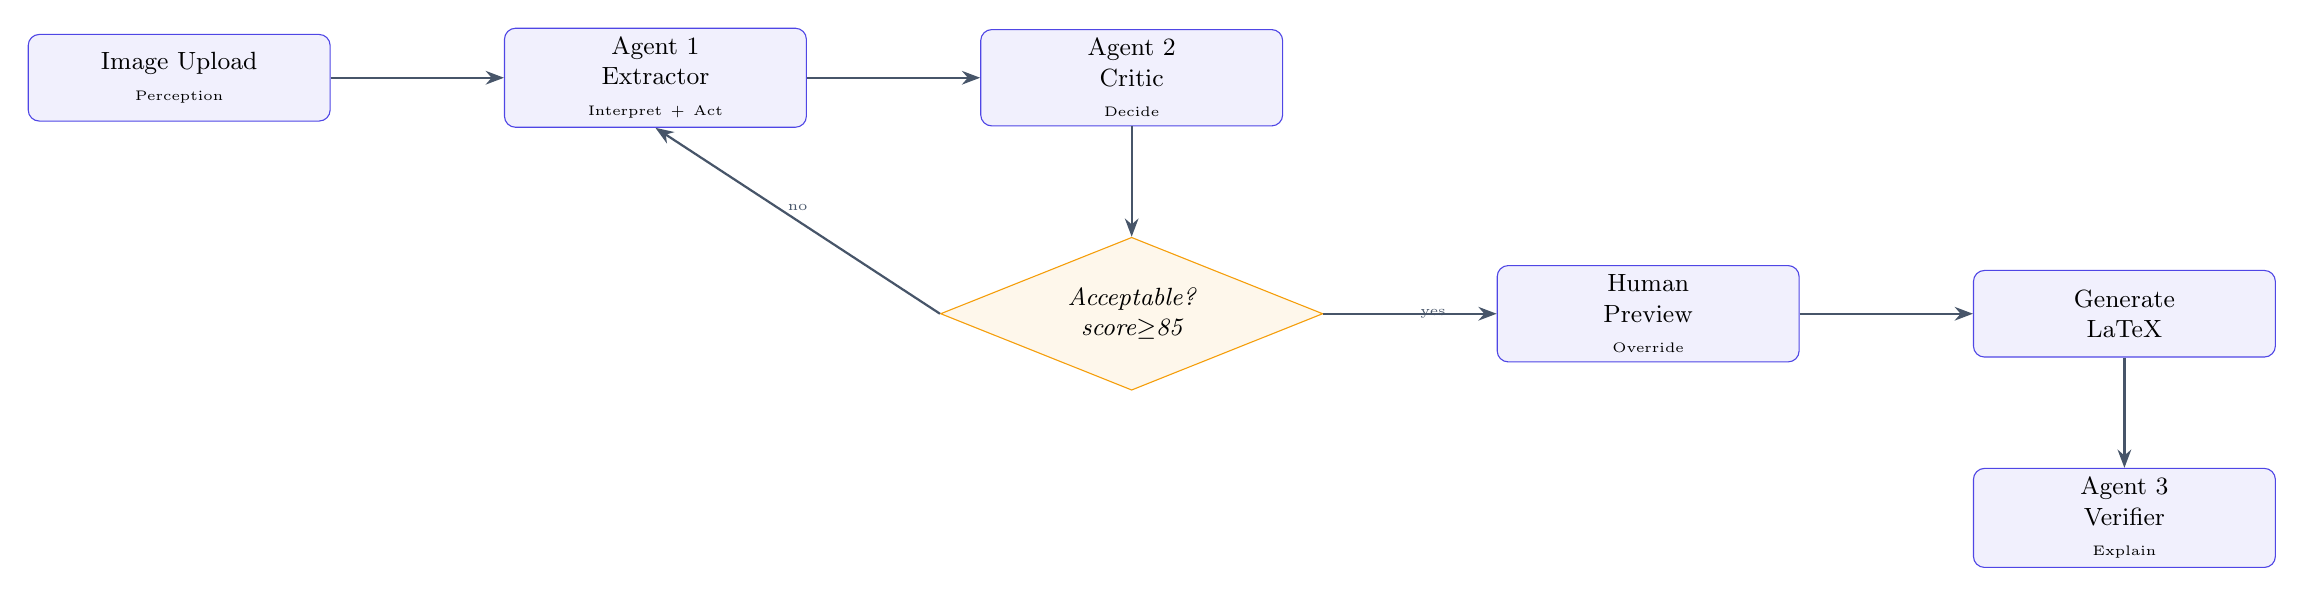
\begin{tikzpicture}[
  node distance=1.4cm and 2.2cm,
  box/.style={rectangle, rounded corners=4pt, draw=indigo, fill=indigo!8,
               text width=3.6cm, align=center, minimum height=1.1cm, font=\small},
  decision/.style={diamond, draw=amber, fill=amber!8, aspect=2.5,
                   text width=2.4cm, align=center, font=\small\itshape},
  arr/.style={-Stealth, thick, color=slate},
]
  \node[box]        (img)     {Image Upload\\{\tiny Perception}};
  \node[box, right=of img]    (a1)  {Agent 1\\Extractor\\{\tiny Interpret + Act}};
  \node[box, right=of a1]     (a2)  {Agent 2\\Critic\\{\tiny Decide}};
  \node[decision, below=of a2](ok)  {Acceptable?\\score$\geq$85};
  \node[box, right=of ok]     (hitl){Human\\Preview\\{\tiny Override}};
  \node[box, right=of hitl]   (gen) {Generate\\LaTeX};
  \node[box, below=of gen]    (a3)  {Agent 3\\Verifier\\{\tiny Explain}};

  \draw[arr] (img)  -- (a1);
  \draw[arr] (a1)   -- (a2);
  \draw[arr] (a2)   -- (ok);
  \draw[arr] (ok)   -- node[right]{\tiny yes} (hitl);
  \draw[arr] (ok.west) -- node[above,font=\tiny]{no} (a1.south);
  \draw[arr] (hitl) -- (gen);
  \draw[arr] (gen)  -- (a3);
\end{tikzpicture}
\end{center}

\subsection{Agent 1 — Extractor (Perception + Action)}
\begin{itemize}[noitemsep]
  \item \textbf{Role:} Perceive the document image and produce a complete structured JSON
    representation of all elements (text, lists, tables, formulas, images).
  \item \textbf{Tool:} \texttt{extract\_document} — a forced-choice Claude tool-use call that
    guarantees structured output.
  \item \textbf{Memory:} On refinement passes, receives the full cumulative critique history
    (all previous pass scores and issues), not just the most recent critique.
  \item \textbf{Hard constraint:} Every visible diagram/image MUST be returned with a bounding
    box. Violation triggers immediate re-extraction.
\end{itemize}

\subsection{Agent 2 — Critic (Decision)}
\begin{itemize}[noitemsep]
  \item \textbf{Role:} Observe both the original image and the current extraction JSON; decide
    whether the quality is acceptable; produce a structured critique.
  \item \textbf{Tool:} \texttt{critique\_extraction} — returns \texttt{quality\_score},
    \texttt{is\_acceptable}, \texttt{issues} (with severity: critical / major / minor),
    \texttt{missing\_content}, and a summary.
  \item \textbf{Decision rules:}
    \begin{itemize}[noitemsep]
      \item \texttt{is\_acceptable = true} only when score $\geq 85$ AND no critical issues AND
        all visible images are accounted for.
      \item Any missing image or missing bbox $\Rightarrow$ \texttt{is\_acceptable = false}
        regardless of score.
    \end{itemize}
\end{itemize}

\subsection{Agent 3 — Verifier (Explainability)}
\begin{itemize}[noitemsep]
  \item \textbf{Role:} After LaTeX generation, compare the original image against the compiled
    LaTeX source and report an accuracy score with specific issues.
  \item \textbf{Tool:} \texttt{report\_verification} — returns \texttt{accuracy\_score},
    categorised issues (high / medium / low severity), missing elements, and a summary.
  \item \textbf{Purpose:} This agent is not part of the extraction loop — it is a
    \emph{post-hoc explainability mechanism} that gives the user an independent audit of the
    final output before they use it.
\end{itemize}

\subsection{Agent Type Selection: Goal-Based + Learning}

The system is a \textbf{goal-based agent}: it has an explicit quality goal (score $\geq 85$,
no critical issues, all images present) and takes actions (refine extraction) to reach that
goal. It also exhibits \textbf{limited learning}: each refinement pass benefits from the
accumulated critique history, meaning the extractor does not repeat the same mistakes across
passes. Full reinforcement-learning-based adaptation is beyond scope but represents a natural
future extension.

\subsection{Operational Workflow: Observe $\rightarrow$ Interpret $\rightarrow$ Decide $\rightarrow$ Act $\rightarrow$ Learn}

\begin{center}
\begin{tabular}{lll}
  \toprule
  \textbf{Step} & \textbf{Agent} & \textbf{Implementation} \\
  \midrule
  Observe    & A1 + A2 & Image encoded as base64, sent to Claude vision API \\
  Interpret  & A1      & Layout detection, element type classification \\
  Decide     & A2      & Quality score calculation; is\_acceptable gate \\
  Act        & A1      & Extraction or targeted refinement based on critique \\
  Learn      & A1      & Cumulative critique history passed on every refinement pass \\
  \bottomrule
\end{tabular}
\end{center}


% =============================================================================
\section{Memory \& Context}
% =============================================================================

\subsection{Short-Term Memory}

\begin{itemize}[noitemsep]
  \item \textbf{Iteration log:} Each pass appends \{\texttt{pass}, \texttt{elements},
    \texttt{critique}\} to an \texttt{iteration\_log} list. This is passed to Agent 1 on every
    refinement pass, giving it full awareness of what was wrong in prior passes.
  \item \textbf{Session store:} An in-memory Python dict (\texttt{sessions[uuid]}) holds the
    extracted data, temp directory, original image copy, filename, timestamp, and user rating
    for the duration of the browser session.
  \item \textbf{Best image elements:} A dedicated list (\texttt{best\_image\_elements}) tracks
    every image element that had a successful crop across all passes. If the model drops an image
    in a later pass, it is automatically restored from this list.
\end{itemize}

\subsection{Long-Term Memory}

Session data is not persisted to disk. A lightweight history list (capped at 20 entries)
stores metadata (filename, timestamp, rating) in memory for the lifetime of the server process.
True long-term memory (database persistence, user accounts) is identified as a future
enhancement.


% =============================================================================
\section{Autonomy Level}
% =============================================================================

The system operates at \textbf{semi-autonomy}:

\begin{itemize}[noitemsep]
  \item \textbf{Autonomous:} The extract/critique/refine loop runs without user intervention,
    up to 4 passes, until the quality gate is satisfied.
  \item \textbf{Human-controlled:} The loop result is \emph{never} automatically committed.
    The user must review and approve all extracted elements in the preview step before LaTeX
    is generated.
\end{itemize}

Full autonomy (automatically generating and delivering the final document) was considered and
\textbf{rejected} on ethical grounds: errors in academic documents can have serious consequences
(incorrect exam answers, corrupted data), and the user must bear ultimate responsibility for the
output they submit.


% =============================================================================
\section{Human-in-the-Loop}
\label{sec:hitl}
% =============================================================================

The Human-in-the-Loop (HitL) gate is the central ethical safeguard of the system. After the
agentic extraction loop converges, the user is presented with the \textbf{Preview Step}:

\begin{itemize}[noitemsep]
  \item Every extracted element is displayed with its type badge, content, and formatting.
  \item The user can: edit any text, change element types, adjust heading levels, toggle bold /
    italic / underline, delete any element, or change the document title.
  \item Image elements show the bounding-box region that will be cropped from the original.
  \item Only after the user clicks ``Generate LaTeX'' does the system proceed.
\end{itemize}

The HitL step \emph{intentionally interrupts} automation. It reflects the
deontological principle that transparency and user control are duties, not optional features.


% =============================================================================
\section{Ethical Agent Design}
% =============================================================================

\begin{center}
\begin{tabular}{lp{10cm}}
  \toprule
  \textbf{Principle} & \textbf{Implementation} \\
  \midrule
  Privacy         & Images are sent to Anthropic's API only for processing; no content is
                    logged or persisted beyond the active session. Temp files are deleted
                    immediately after extraction. \\[0.4em]
  Bias mitigation & Agent 1 and Agent 2 use different system roles and incentives to reduce
                    single-model bias. Agent 2 is explicitly instructed to be stricter than
                    Agent 1. \\[0.4em]
  Transparency    & All agent decisions are streamed to the UI in real time. Users can see
                    every pass, every score, and every critique issue as they happen. \\[0.4em]
  User control    & The HitL preview step, the ability to override any AI decision, and the
                    Agent 3 verification report give the user full control at every stage. \\
  \bottomrule
\end{tabular}
\end{center}


% =============================================================================
\section{Risk Assessment}
% =============================================================================

\begin{center}
\begin{tabular}{p{3.5cm}p{4cm}p{4.5cm}l}
  \toprule
  \textbf{Risk} & \textbf{Description} & \textbf{Mitigation} & \textbf{Severity} \\
  \midrule
  Incorrect decisions &
    Agent 2 incorrectly accepts a poor extraction &
    User preview + Agent 3 verification provide two additional checkpoints &
    Medium \\[0.4em]
  Over-automation &
    Users blindly accept AI output without review &
    Mandatory HitL preview; Agent 3 score visible before use &
    Medium \\[0.4em]
  Misuse &
    Tool used to transcribe copyrighted content &
    No server-side content filtering is implemented (out of scope) &
    Low \\[0.4em]
  API key exposure &
    Key leaked via logs or version control &
    \texttt{.env} + \texttt{.gitignore}; key never transmitted to frontend &
    High \\[0.4em]
  Image data leakage &
    Sensitive images exposed via API &
    In-memory sessions; temp files deleted; no external logging &
    Medium \\
  \bottomrule
\end{tabular}
\end{center}


% =============================================================================
\section{Safety Mechanisms}
% =============================================================================

\begin{enumerate}[noitemsep]
  \item \textbf{Logging:} Every agent action (pass number, element count, critique score) is
    logged server-side with timestamps using Python's \texttt{logging} module at INFO level.

  \item \textbf{Override (Human-in-the-Loop):} The user can override any AI decision in the
    preview step before LaTeX generation.

  \item \textbf{Explainability:} Agent 3 provides a post-hoc verification report with a
    numerical accuracy score and categorised issues, displayed in the UI with severity badges.

  \item \textbf{Image preservation safety net:} A \texttt{best\_image\_elements} list persists
    all successfully cropped images across passes. If Agent 1 drops an image in a later
    refinement, it is automatically restored before the result is shown.

  \item \textbf{Max passes cap:} The agentic loop is hard-capped at 4 passes to prevent
    infinite loops and uncontrolled API spending.

  \item \textbf{Convergence condition:} Early exit when quality is acceptable prevents
    unnecessary passes and reduces both latency and cost.
\end{enumerate}


% =============================================================================
\section{Legal Aspects of Computing}
% =============================================================================

\subsection{Developer Responsibilities: Data Protection \& User Rights}

As a developer processing user-uploaded documents, the following legal obligations apply:

\begin{itemize}[noitemsep]
  \item \textbf{Data minimisation:} Only the data necessary for processing (the image) is
    transmitted. No user accounts, email addresses, or additional personal data are collected.
  \item \textbf{Right to erasure:} Sessions are in-memory and cleared when the server restarts.
    Users can reset their session at any time.
  \item \textbf{Transparency:} Users should be informed that images are processed by Anthropic's
    API. This is a known limitation of the current implementation.
\end{itemize}

\subsection{PECA 2016 — Computer Crimes \& Risks}

Pakistan's Prevention of Electronic Crimes Act 2016 is relevant to this project in the
following ways:

\begin{itemize}[noitemsep]
  \item \textbf{Unauthorised access (Sec 3):} The API key must be protected. If exposed, a
    third party could use it to make API calls on the developer's account — constituting
    unauthorised use of a computing resource.
  \item \textbf{Data interference (Sec 6):} The system must not alter user-uploaded images
    beyond the explicitly described processing (resizing for API, cropping for output). Any
    undisclosed manipulation would be legally problematic.
\end{itemize}

\subsection{Computer Contracts: Terms of Service}

By using Anthropic's Claude API, the developer accepts:
\begin{itemize}[noitemsep]
  \item Anthropic's usage policies (no harmful content generation, no misuse for academic
    dishonesty facilitation).
  \item Data processing terms: images are not used for model training without explicit consent
    (per Anthropic's API terms as of 2025).
  \item Rate limiting and fair use: the application must not implement automated bulk processing
    that violates API quotas.
\end{itemize}


% =============================================================================
\section{Intellectual Property Rights}
% =============================================================================

\begin{itemize}[noitemsep]
  \item \textbf{Ownership of this application:} The code, prompt engineering, and system
    architecture are original work. The application does not incorporate licensed third-party
    code beyond open-source libraries (MIT/Apache licensed: FastAPI, React, Tailwind, Pillow,
    Anthropic SDK).

  \item \textbf{IPR of processed content:} The tool transcribes documents but does not claim
    any rights over the content. Copyright of the original document remains with its author.

  \item \textbf{GDPR mindset — data protection awareness:}
    \begin{itemize}[noitemsep]
      \item Images are \emph{personal data} if they contain identifiable information.
      \item Processing is lawful only if the user has consented (implicit in their upload action).
      \item The processor (this application) must not retain data beyond the stated purpose
        (session-scoped processing).
    \end{itemize}

  \item \textbf{Licensing options:} If open-sourced, this project would be released under the
    MIT License, consistent with its dependency stack.
\end{itemize}


% =============================================================================
\section{Career Relevance}
% =============================================================================

\subsection{Skills Developed}

\begin{multicols}{2}
\begin{itemize}[noitemsep]
  \item Multi-agent system design
  \item LLM prompt engineering
  \item Structured tool-use (JSON schema)
  \item Server-Sent Events (SSE) streaming
  \item Async Python (FastAPI + asyncio)
  \item React + TypeScript frontend
  \item LaTeX document generation
  \item Ethical agent design
  \item Professional risk assessment
  \item Legal awareness in software
\end{itemize}
\end{multicols}

\subsection{Industry Relevance in the Agentic AI Era}

The shift toward agentic AI is the defining industry trend of 2024--2026. Companies including
Anthropic, OpenAI, Google DeepMind, and Microsoft are investing heavily in multi-agent
frameworks. Graduates who understand:
\begin{itemize}[noitemsep]
  \item How to design critique-and-refine loops
  \item How to enforce quality gates in autonomous systems
  \item How to maintain human oversight in AI pipelines
  \item How to apply ethical frameworks to AI decision-making
\end{itemize}
will be significantly more competitive than those who can only call an API and display the
result.


% =============================================================================
\section{Virtual Work \& Sustainability}
% =============================================================================

\subsection{Remote Collaboration}
This project was developed using:
\begin{itemize}[noitemsep]
  \item \textbf{Git} for asynchronous version control (no physical co-location required)
  \item \textbf{Vite dev server} with remote host support (\texttt{--host 0.0.0.0}) enabling
    testing from any device on the network
  \item \textbf{A \texttt{manage.sh} script} that standardises the development environment
    startup, reducing onboarding time for remote collaborators
\end{itemize}

\subsection{Green Computing: Efficient Resource Use}
\begin{itemize}[noitemsep]
  \item \textbf{Early convergence:} The loop exits as soon as quality is acceptable, minimising
    unnecessary API calls (each of which consumes energy at Anthropic's data centres).
  \item \textbf{Image resizing:} Only a 1568px-max version of the image is sent to the API;
    the original is kept locally for high-quality cropping. This reduces data transfer and
    API processing cost.
  \item \textbf{Prompt caching:} Claude's \texttt{cache\_control: ephemeral} is applied to
    tool definitions and system prompts, reducing token re-processing on subsequent calls.
  \item \textbf{Tectonic over TeX Live:} Tectonic downloads only the packages needed for each
    document, rather than installing a multi-gigabyte full TeX distribution.
\end{itemize}


% =============================================================================
\section{Comparative Analysis: Phase 1 vs.\ Phase 2}
% =============================================================================

\begin{center}
\begin{longtable}{lp{5cm}p{5.5cm}}
  \toprule
  \textbf{Feature} & \textbf{Phase 1} & \textbf{Phase 2 (Agentic)} \\
  \midrule
  Architecture    & Single-pass pipeline & Multi-agent loop (A1 $\leftrightarrow$ A2 $\rightarrow$ A3) \\
  Control         & User-driven (request/response) & System-driven (autonomous until quality gate) \\
  Intelligence    & Static (single prompt) & Adaptive (critique $\rightarrow$ refine) \\
  Behaviour       & Reactive & Proactive \\
  Memory          & None & Short-term (iteration log, best images) \\
  Image handling  & Single crop attempt; silent drop on failure & Multi-pass with safety net; placeholder on failure \\
  Progress        & Spinner (opaque) & Real-time SSE stream with per-agent messages \\
  Quality assurance & None & Agent 2 critique score + Agent 3 verification \\
  Human oversight & None (direct output) & Mandatory preview + override \\
  Ethical design  & Implicit & Explicit (transparency, privacy, override, explainability) \\
  \bottomrule
  \caption{Phase 1 vs.\ Phase 2 comparative analysis}
\end{longtable}
\end{center}


% =============================================================================
\section{Conclusion}
% =============================================================================

Phase 2 of Layout OCR represents a genuine transformation from a static tool to a purposefully
designed agentic system. The core contribution is not the use of AI — Phase 1 used AI too —
but the \emph{structure} of how AI is used:

\begin{enumerate}[noitemsep]
  \item A dedicated \textbf{critic agent} that enforces quality standards the generator might
    not meet alone.
  \item A \textbf{memory layer} that accumulates critique history so errors are not repeated.
  \item A \textbf{safety net} that preserves information (image elements) against model
    regression across passes.
  \item A \textbf{human gate} that ensures no AI decision is irreversible without user
    approval.
  \item A \textbf{verifier agent} that explains the final output quality after the fact.
\end{enumerate}

These design decisions were not made for technical novelty. They were made because academic
document transcription is \textbf{high-stakes}, because AI systems are \textbf{imperfect}, and
because professional software engineering demands that we \textbf{design for failure, not just
for success}.

The system embodies the principle that outstanding agentic design means ``redesigning
decision-making systems, addressing ethical risks of autonomy, and demonstrating professional
responsibility'' — not simply adding an API call.

\vspace{1cm}
\begin{successbox}
\textbf{Alignment with NCEAC Learning Outcomes:}
\begin{itemize}[noitemsep]
  \item \textbf{CLO 4} — Ethical reasoning demonstrated throughout agent design and HitL
    decisions
  \item \textbf{CLO 5} — IPR analysis of application ownership and content processing
  \item \textbf{CLO 6} — PECA 2016 risk analysis; data protection awareness; API terms review
  \item \textbf{CLO 8} — Industry trends analysis; career skill mapping; green computing
\end{itemize}
\end{successbox}

\end{document}
